\documentclass[../sparc.tex]{subfiles}
\graphicspath{{\subfix{../images/}}}
\begin{document}

%%%%%%%%%%%%%%%%%%%%%%%%%%%%%%%%%%%%%%%%%%%%%%%%%%%%%%%%%%%%%%%%%%%%%%%%%%%%%%%%
\section{Building Electric Circuits}

It would be hard to talk about modern digital circuitry without mentioning a
\emph{micro-controller} -- it is a ``brain'' of many systems that we interact
with each day.

A micro-controller is a simple and usually quite cheap embedded computer often
built to solve one task.  Micro-controllers are in control (pun intended) of
many modern household appliances, children toys, electronic musical instruments
and factory robots; 3D-printers and other CNCs are built upon micro-controllers.

We will be working with Arduino platform that is widely available and provides
convenient interface for the practical application and programming.

Its appearance may vary depending on the model; you can find a photo of one of
the popular Arduino model called ``Arduino UNO'' on
fig. \ref{fig:arduino-uno-r3}.

\begin{figure}[ht]
  \centering
  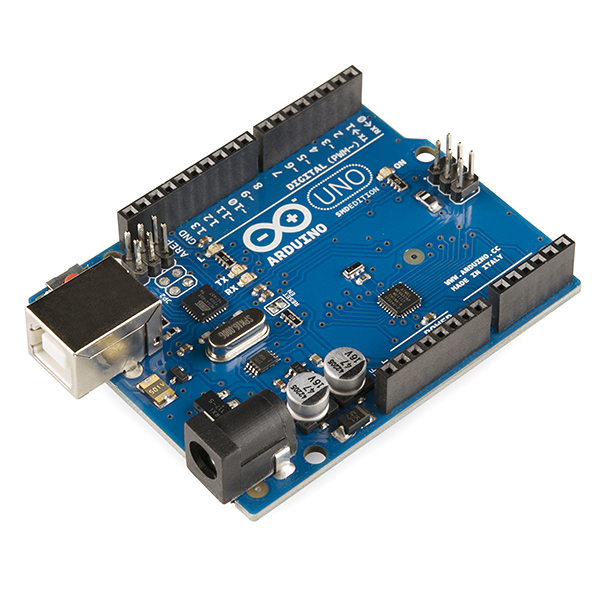
\includegraphics[width=12cm]{Arduino_Uno_-_R3}
  \caption{Micro-controller platform ``Arduino UNO'' R3.}
  \label{fig:arduino-uno-r3}
\end{figure}

We will discuss Arduino usage and programming in the chapter
\ref{chapter:dialogues-with-computer}.  Meanwhile we will use Arduino simply as
the voltage source in the place of a battery in our circuits.

As shown on fig. \ref{fig:arduino-uno-r3} Arduino has special connectors that
are called \emph{ports} that allow us to connect external components and wires
to the board.  Some ports are numbered as 0, 1, 2 etc. -- those are \emph{digital
ports}.  Also you can find ports labeled as ``A0'', ``A1'', ``A2'' etc. -- and
they are called \emph{analog ports}.  We won't be using digital and analog ports
in this chapter as we will need to write some program for our micro-controller
to work with them; and that's a topic for another chapter.

Now please note two Arduino ports labeled as ``GND'' and ``5V''.

``GND'' means ``Ground'' -- this is a port that always has 0V on it.  ``5V'' is
always have 5V as you probably already guessed.

Let's build an electric circuit with a resistor and an LED shown on
fig. \ref{fig:electronics-arduino-circuit-00}.

\begin{figure}[ht]
  \centering
  \begin{circuitikz}
    \draw (3.5, 0) node[
      dipchip,
      num pins=2,
      external pins width=0.0,
      no topmark,
      hide numbers,
      xscale = 2.5,
      yscale = 2.5](C1){Arduino};
    \node [above left, font=\small] at (C1.bpin 1) {5V};
    \node [above right, font=\small] at (C1.bpin 2) {GND};
    \draw
    (C1.bpin 1) to[short]
    (0, 0) to[short]
    (0, 4) to[resistor, l=$R_1$] (3, 4)
    (3, 4) to[full led, l=LED] (7, 4)
    (7, 4) to[short]
    (7, 0) to[short]
    (C1.bpin 2);
  \end{circuitikz}
  \caption{A circuit with a resistor, an LED and Arduino.}
  \label{fig:electronics-arduino-circuit-00}
\end{figure}

We will assembly our circuit using a \emph{breadboard}.  The appearance of a
breadboard is shown on fig. \ref{fig:breadboard}.  On the left side of the
figure you can see the front view of a breadboard, where electronic components
and wires are inserted during circuit assembly.  On the right side, the rear
side of a breadboard is shown.  Usually the rear side is covered with a piece of
two-side adhesive tape with a protective layer on top -- this way you can glue
the breadboard somewhere if you need it.  On the breadboard shown on
fig. \ref{fig:breadboard} this adhesive layer is removed to show the breadboard
insides; you shouldn't remove this adhesive layer without good reasons to do it
as this layer also provides an insulation for the conductors inside the
breadboard.

\begin{figure}[ht]
  \centering
  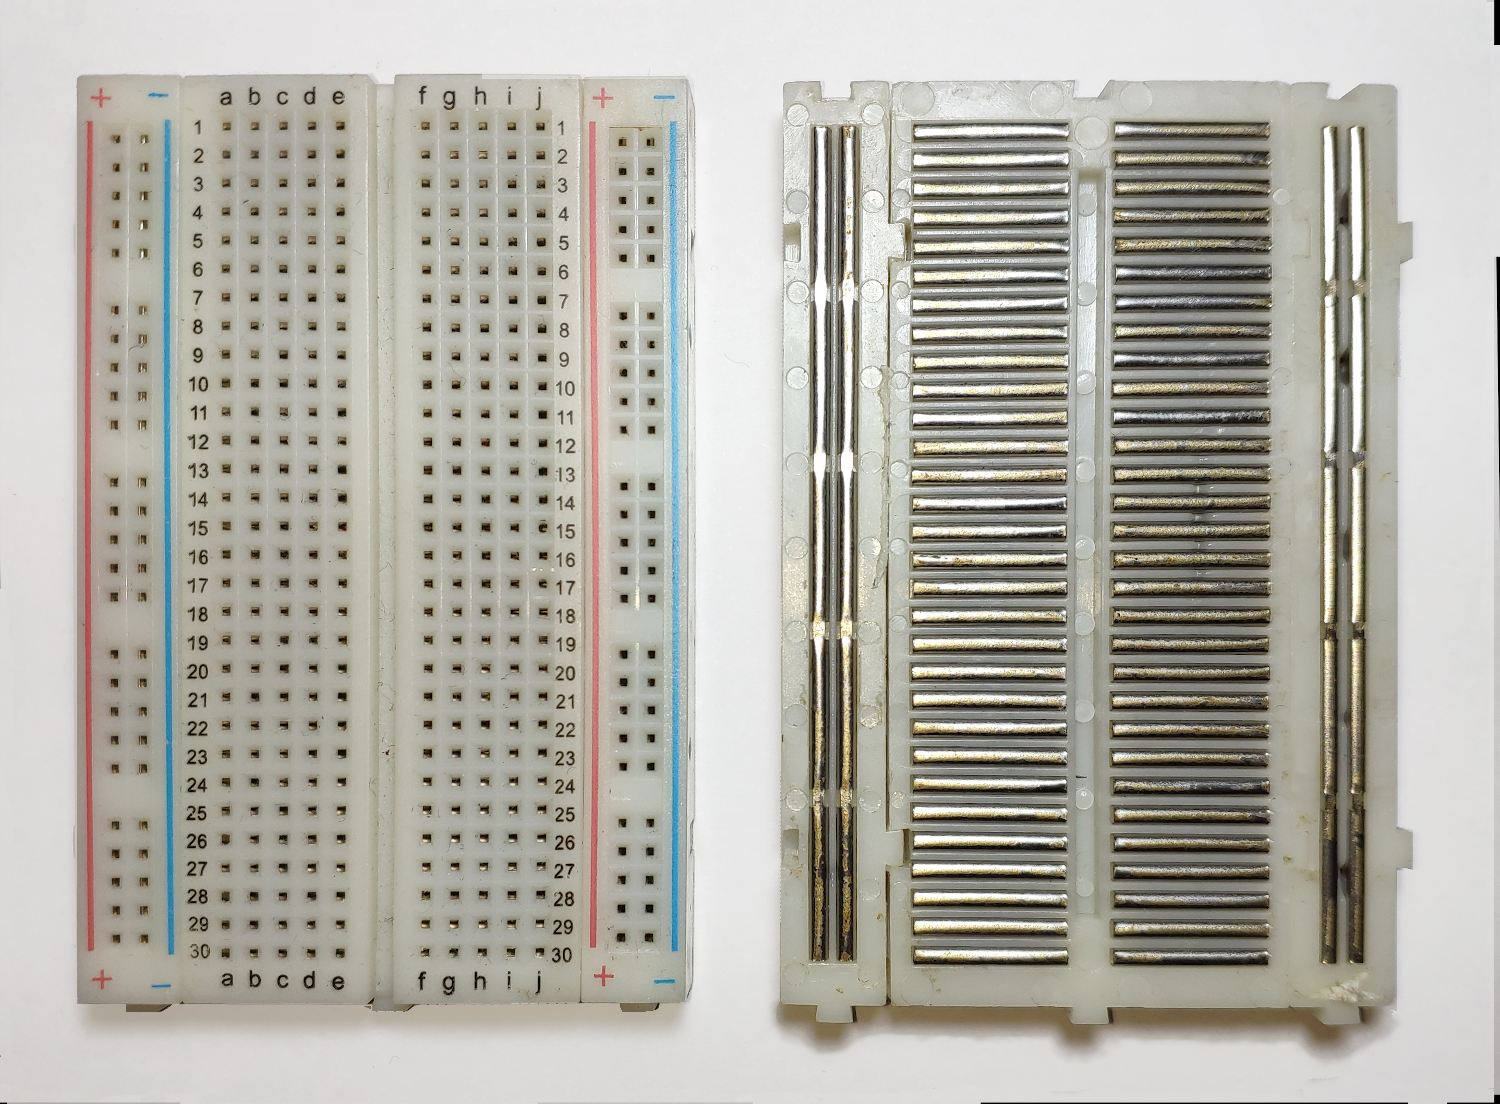
\includegraphics[width=12cm]{Breadboard}
  \caption{A breadboard.}
  \label{fig:breadboard}
\end{figure}

As you can see on fig. \ref{fig:breadboard} a breadboard is but a piece of
plastic with metallic inserts that provide connections between electronic
components of a circuit built upon a breadboard.

Across the breadboard on each side you can find a pair of long lines that are
marked on the front of the breadboard with symbols ``+'' and ``-'' -- they
usually are used for providing common ground and power lines for a circuit.

An example of an electric circuit built on a breadboard is shown on
fig. \ref{fig:breadboard-simple-arduino-circuit}.

\begin{figure}[ht]
  \centering
  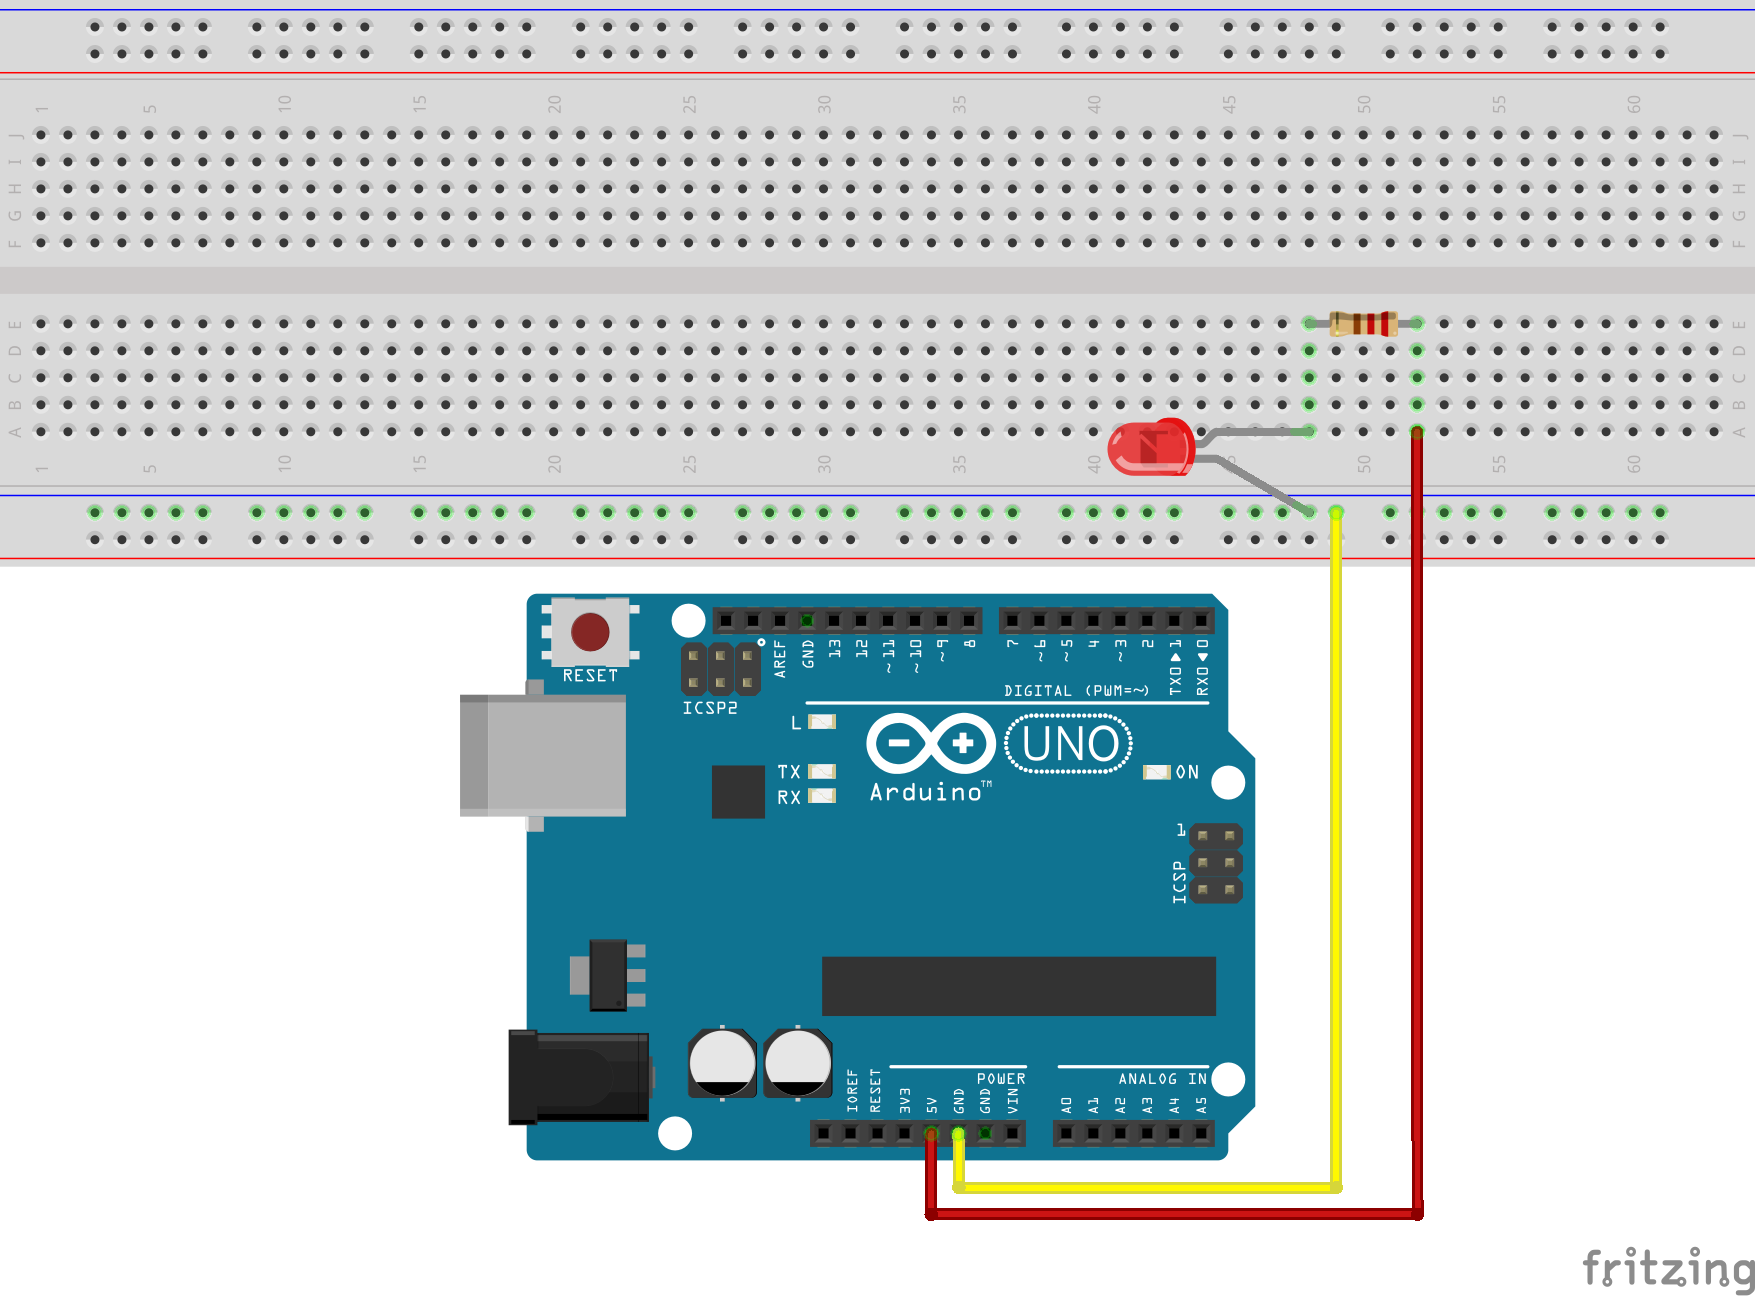
\includegraphics[width=12cm]{schematics/002-simple-arduino-circuit}
  \caption{An example of an electric circuit with an LED and a resistor that
    uses Arduino UNO as the power supply.}
  \label{fig:breadboard-simple-arduino-circuit}
\end{figure}

Note that the resistance value for $R_1$ should be not less than 200 Ohms.

Carefully check the circuit before powering up the Arduino.  First of all
closely inspect the two wires that go from Arduino to the breadboard -- they must
not be connected directly with each other.  You can see on
fig. \ref{fig:breadboard-simple-arduino-circuit} that one wire connects Arduino
5V port to one of the resistor legs and another wire goes from GND (GROUND) to a
common ``-'' line on the breadboard marked by blue color where the LED cathode
is connected.

After powering up the Arduino the LED should light up.  If this does not happen
then you should power off the Arduino and check the schematics again.  One of
the common reasons why an LED is not working, is due to mixed up anode and
cathode connection of the LED; in that case all you need is to switch LED legs
on the breadboard.

\experiment{0}{Try to replace $R_1$ resistor with another one with higher
  resistance (e.g. 500 Ohms.)  How the brightness of the LED is changed?}

Now we will try to make a serial connection of resistors.  Let's use for the
task two resistors with values 200 and 300 Ohms and build our new circuit with
that as shown on fig. \ref{:electronics-arduino-circuit-00}.

\begin{figure}[ht]
  \centering
  \begin{circuitikz}
    \draw (4, 0) node [
      dipchip,
      num pins=2,
      external pins width=0.0,
      no topmark,
      hide numbers,
      xscale = 2.5,
      yscale = 2.5
    ](C1){Arduino};
    \node [above left, font=\small] at (C1.bpin 1) {5V};
    \node [above right, font=\small] at (C1.bpin 2) {GND};
    \draw
    (C1.bpin 1) to[short]
    (0, 0) to[short]
    (0, 4) to[resistor, l=$R_1$] (3, 4)
    (3, 4) to[resistor, l=$R_2$] (6, 4)
    (6, 4) to[full led, l=LED] (8, 4)
    (8, 4) to[short]
    (8, 0) to[short]
    (C1.bpin 2);
  \end{circuitikz}
  \caption{An electronic circuit with an Arduino, LED and two resistors
    connected in the serial manner.}
  \label{fig:electronics-arduino-circuit-00}
\end{figure}

If $R_1$ value is 200 Ohms and $R_2$ value is 300 Ohms then total resistance of
the circuit will be 500 Ohms as per equation
\ref{equation:elemctronics-resistance-0}.

Final circuit is shown on fig.
\ref{fig:breadboard-simple-arduino-circuit-resistor-in-series}.

\begin{figure}[ht]
  \centering
  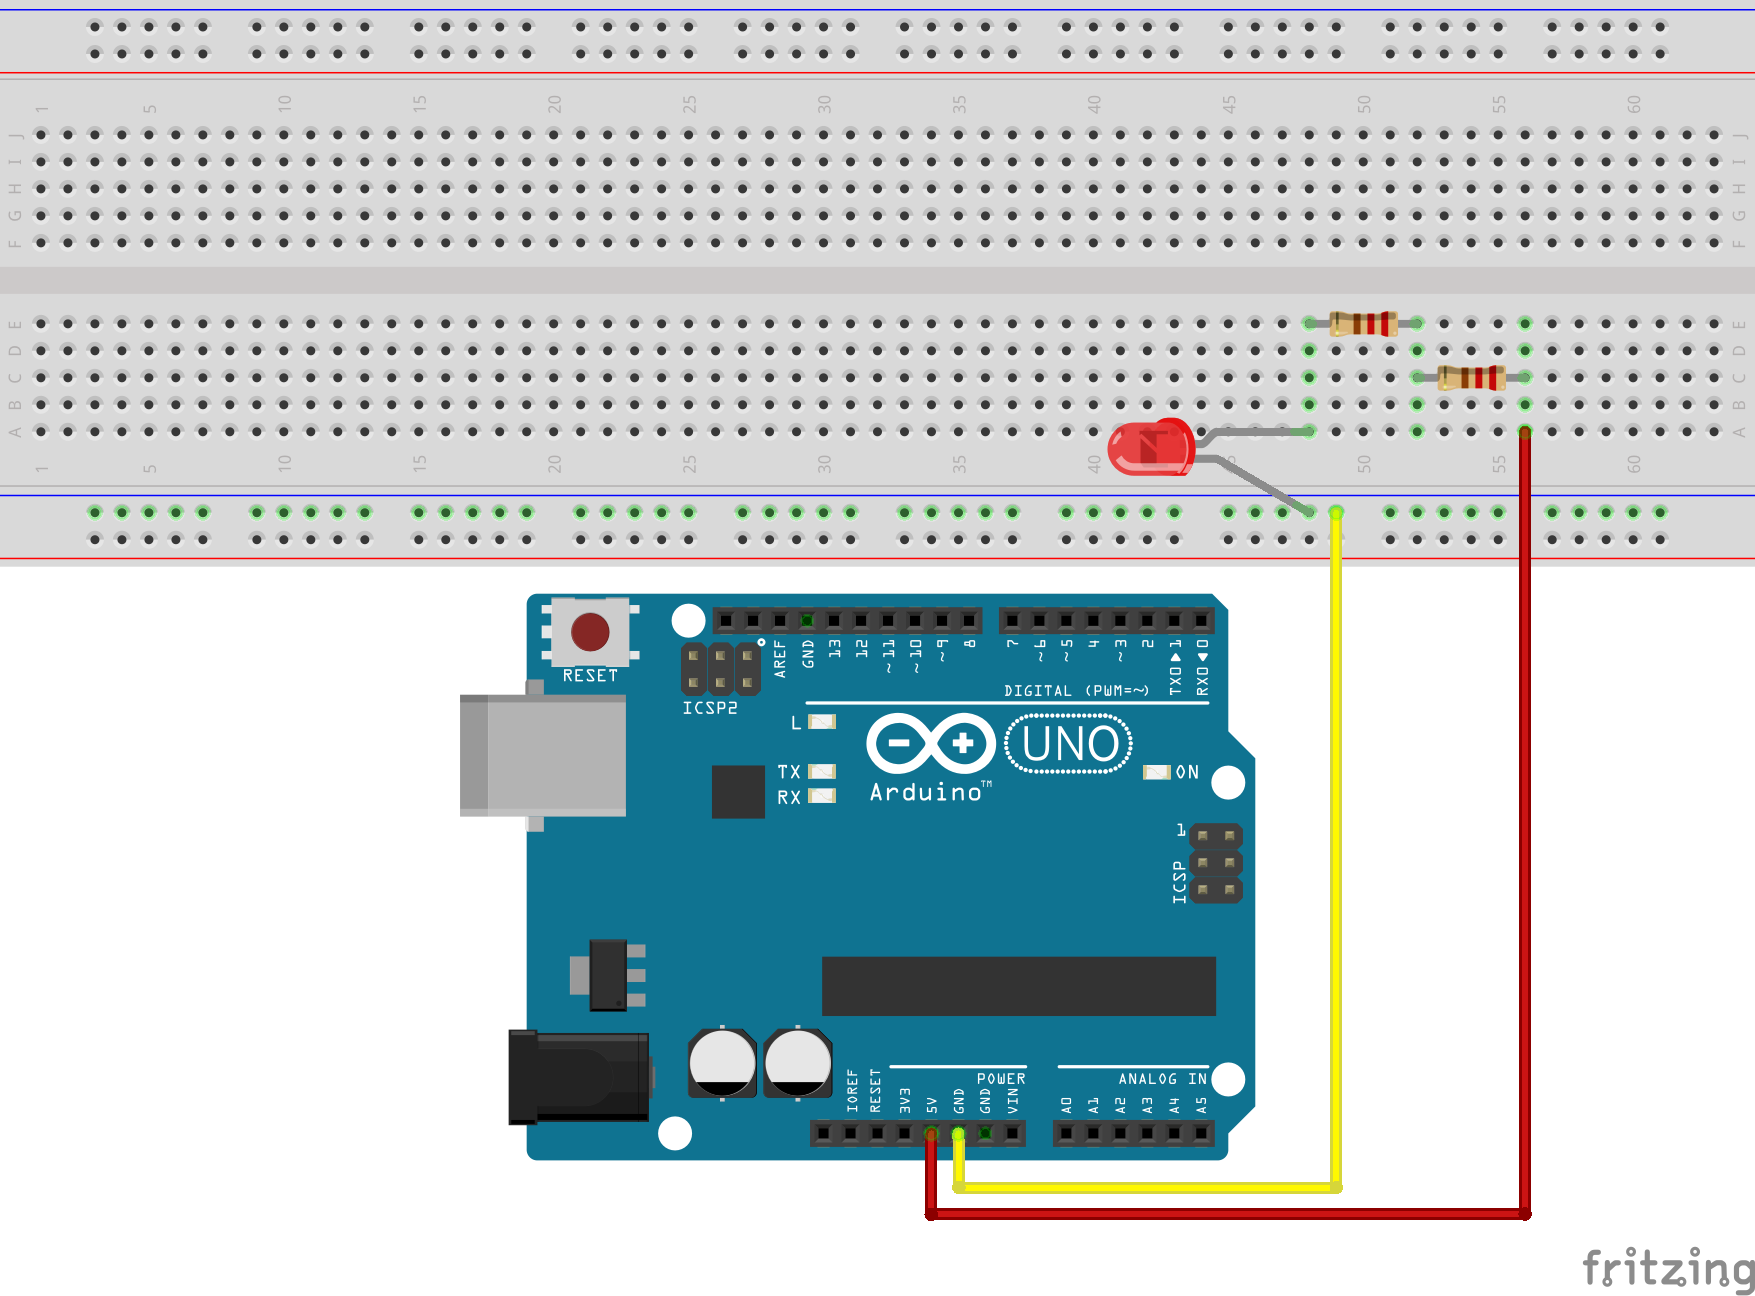
\includegraphics[width=12cm]{schematics/003-simple-arduino-circuit-resistor-in-series}
  \caption{An example of an electric circuit built on a breadboard with an LED
    and two resistors that are connected in serial manner.}
  \label{fig:breadboard-simple-arduino-circuit-resistor-in-series}
\end{figure}

\end{document}
